\section{Similarity Search Case Study}
\label{sec:sampling}

To tackle workload-aware DR, we first perform a case study focusing on time series similarity search by revisiting a widely cited empirical comparison of DR techniques from VLDB 2008~\cite{keogh-study}. 
We show that PCA can outperform classic techniques (return low $k$), but at a high computational cost ($R$).
We then demonstrate how sample-based PCA methods can bridge this gap, but that the number of samples required varies per dataset.
Finally, we show how progressively increasing the sampling rate can help dynamically identify how much to sample a given dataset, thus providing a foundation for workload-aware DR.

\subsection{PCA Speed vs. Quality}

While improved quality provides faster repeated query execution, the cost of DR via PCA dominates this speedup, encouraging the use of faster, lower-quality alternatives~\cite{keogh-study}. 

To briefly quantify this trade-off, we augment a widely-cited time series similarity search DR study from VLDB 2008~\cite{keogh-study} by evaluating PCA---which the authors did not benchmark due to it being ``untenable for large data sets." 
We compare PCA via SVD to baseline techniques based on runtime and DR performance with respect to $TLB$ over the largest datasets from~\cite{keogh-study}. 
We use their two fastest methods as our baselines as they show the remainder exhibited ``very little difference'': Fast Fourier Transform (FFT) and Piecewise Aggregate Approximation (PAA).

\minihead{TLB Performance Comparison}
We compute the minimum dimensionality achieved by each technique subject to a $TLB$ constraint. 
On average, PCA provides bases that are $2.3\times$ (up to $3.9\times$) and $3.7\times$ (up to $26\times$)  smaller than PAA and FFT for $TLB = 0.75$, and $2.9\times$ (up to $8.3\times$) and $1.8\times$ (up to $5.1\times$) smaller for $TLB = 0.99$.
While the margin between PCA and alternatives is dataset-dependent, PCA almost always preserves $TLB$ with a lower dimensional representation.

%\section{Additional End-to-End Plots}
%\input{endendplots}

\minihead{Runtime Performance Comparison} 
PCA implemented via out-of-the-box SVD is on average over \red{$26\times$ (up to $56\times$)} slower than PAA and over \red{$4.6\times$ (up to $9.7\times$)} times slower than FFT when computing the smallest $TLB$-preserving basis.
%This substantiates the observation that classic PCA is incredibly slow compared to alternatives~\cite{keogh-study}. 


\subsection{Incremental, Progressive Sampling}
To bridge this performance-runtime gap, we turn to data sampling. 
Many real-world \red{datasets} are intrinsically low-dimensional, as evidenced by their rapid falloff in their eigenvalue spectrum.
A data sample thus captures much of the dataset's ``interesting'' behavior, so fitting models over data samples generalize well. 
We verify this by varying the target $TLB$ and examining the minimum number of uniformly selected samples required to obtain a $TLB$-preserving transform with output dimension $k$ equal to input dimension $\dvar$.

On average, a sample of under $0.64\%$ $(\text{up to } 5.5\%)$ of the input is sufficient for $TLB = 0.75$, and under $4.2\%$ $(\text{up to } 38.6\%)$ is sufficient for $TLB=0.99$.  
If this sample rate is known, we obtain up to \red{$91\times$ speedup} compared to a na\"ive implementation of PCA via SVD---with no algorithmic improvement. 

However, this benefit is dataset-dependent, and unknown a priori.
We thus turn to progressive sampling (gradually increasing the sample size) to identify how large a sample suffices.
Figure~\ref{fig:progressive} shows how the dimensionality required to attain a given $TLB$ changes when we vary dataset and proportion of data sampled.
Increasing the number of samples provides lower dimensional transformations for the same quality.
However, this decrease in dimension plateaus as the number of samples increases.
Thus, while progressive sampling would allow us to tune the amount of time spent on DR, we must determine when the downstream value of decreased dimension is overpowered by the cost of additional DR---that is, whether to sample to convergence (evaluated in Section~\ref{subsec:lesion}) or terminate early (e.g., at $0.3$ proportion of data sampled for SmallKitchenAppliances). 

\begin{figure}
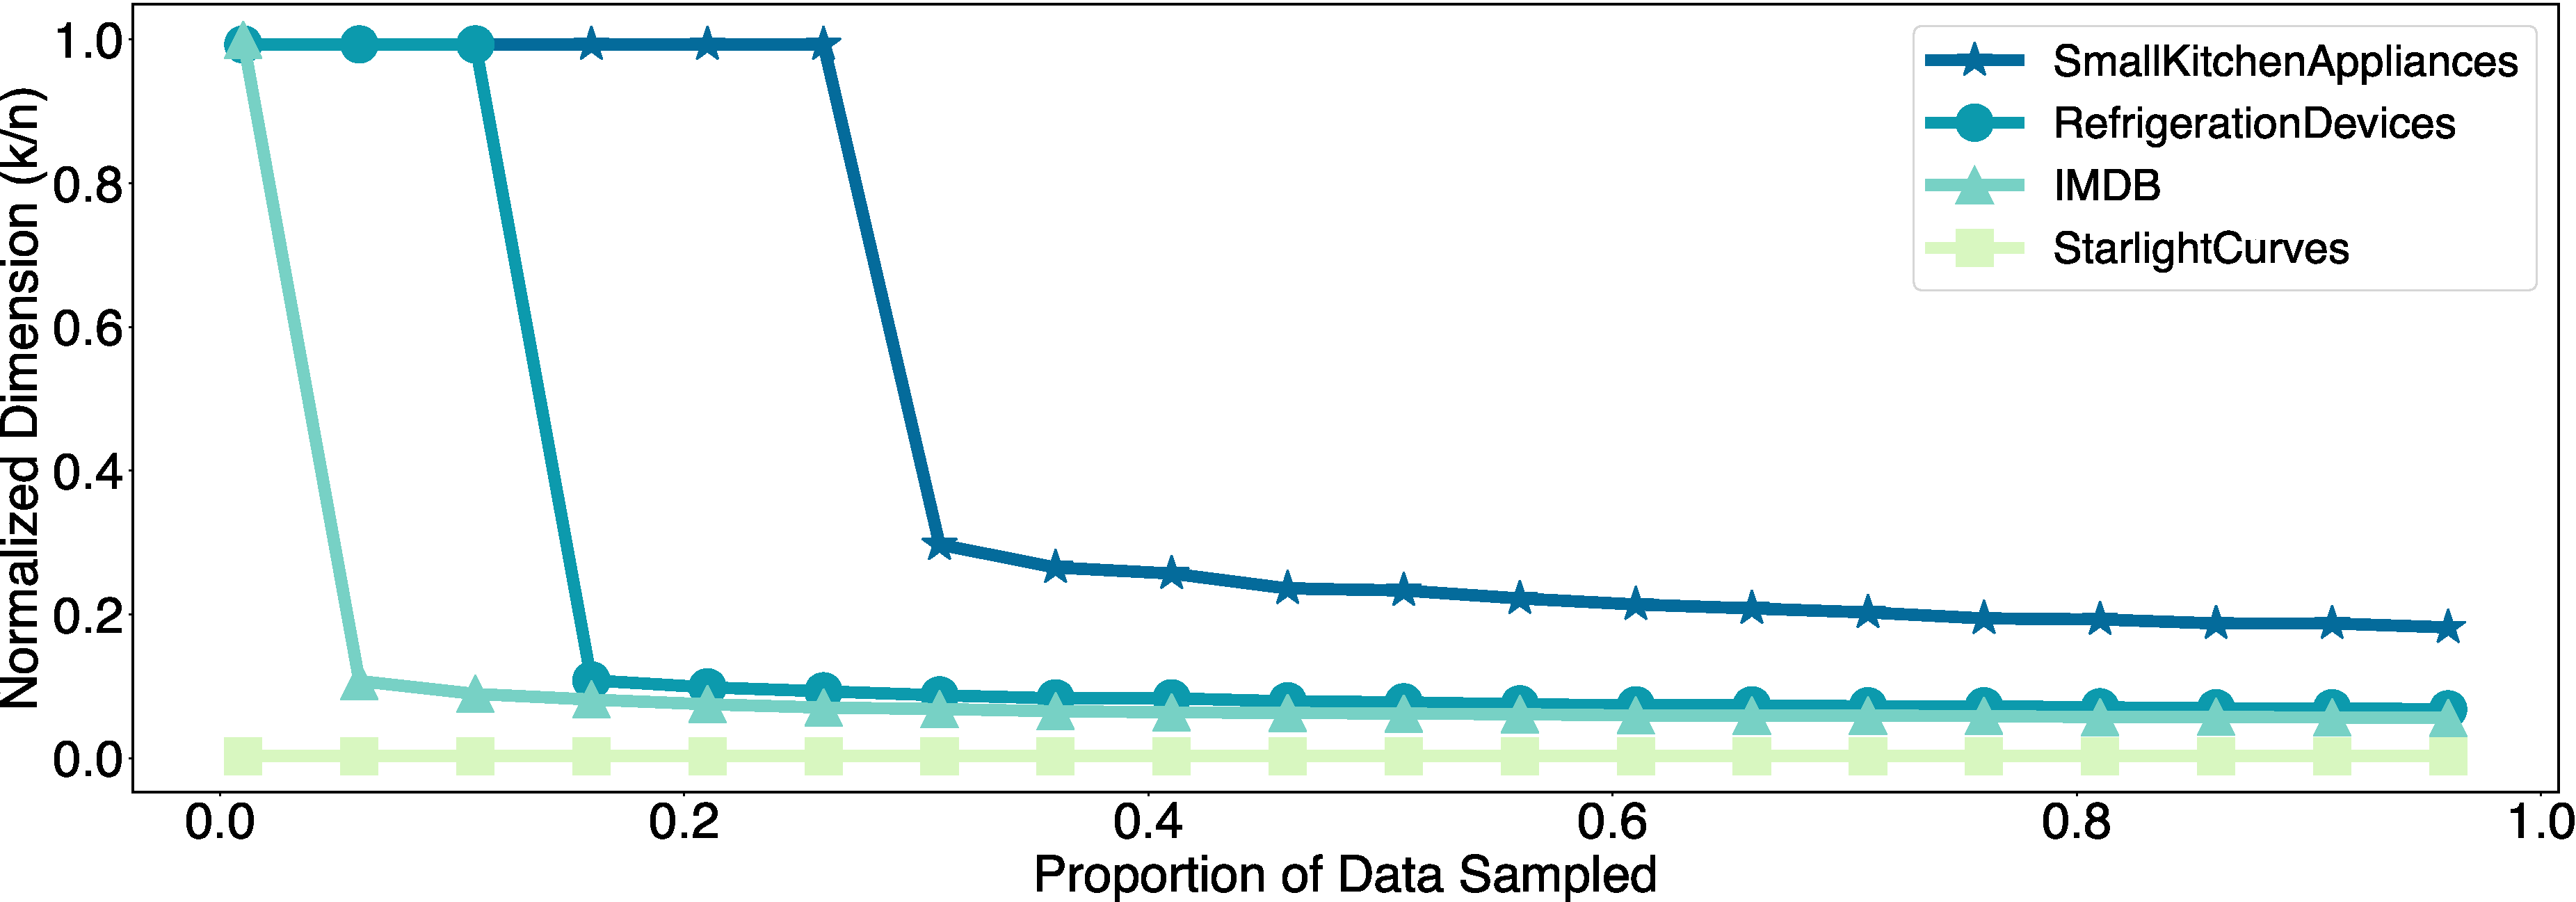
\includegraphics[width=\linewidth]{figs/progressive.pdf}
\caption[]{ Improvement in representation size for  $TLB = 0.80$ across three datasets. Higher sampling rates improve quality until reaching a state equivalent to running PCA over the full dataset ("convergence")}
\label{fig:progressive}
\end{figure}



